%% Преамбула TeX-файла

% 1. Стиль и язык
\documentclass[utf8, 12pt]{G7-32} % Стиль (по умолчанию будет 14pt)

% Остальные стандартные настройки убраны в preamble.inc.tex.
\sloppy

% Настройки стиля ГОСТ 7-32
% Для начала определяем, хотим мы или нет, чтобы рисунки и таблицы нумеровались в пределах раздела, или нам нужна сквозная нумерация.
\EqInChapter % формулы будут нумероваться в пределах раздела
\TableInChapter % таблицы будут нумероваться в пределах раздела
\PicInChapter % рисунки будут нумероваться в пределах раздела
\usepackage{slashbox}

% Добавляем гипертекстовое оглавление в PDF
\usepackage[
bookmarks=true, colorlinks=true, unicode=true,
urlcolor=black,linkcolor=black, anchorcolor=black,
citecolor=black, menucolor=black, filecolor=black,
]{hyperref}

% Изменение начертания шрифта --- после чего выглядит таймсоподобно.
% apt-get install scalable-cyrfonts-tex

\IfFileExists{cyrtimes.sty}
    {
        \usepackage{cyrtimespatched}
    }
    {
        % А если Times нету, то будет CM...
    }

\usepackage{graphicx}   % Пакет для включения рисунков

% С такими оно полями оно работает по-умолчанию:
% \RequirePackage[left=20mm,right=10mm,top=20mm,bottom=20mm,headsep=0pt]{geometry}
% Если вас тошнит от поля в 10мм --- увеличивайте до 20-ти, ну и про переплёт не забывайте:
\geometry{right=20mm}
\geometry{left=30mm}


% Пакет Tikz
\usepackage{tikz}
\usetikzlibrary{arrows,positioning,shadows}

% Произвольная нумерация списков.
\usepackage{enumerate}

% ячейки в несколько строчек
\usepackage{multirow}

% itemize внутри tabular
\usepackage{paralist,array}

% Центрирование подписей к плавающим окружениям
\usepackage[justification=centering]{caption}

% объявляем новую команду для переноса строки внутри ячейки таблицы
\newcommand{\specialcell}[2][c]{%
	\begin{tabular}[#1]{@{}c@{}}#2\end{tabular}}



% Настройки листингов.
\ifPDFTeX
% Листинги

\usepackage{listings}
\usepackage{wrapfig}
% Значения по умолчанию
\lstset{
  basicstyle= \footnotesize,
  breakatwhitespace=true,% разрыв строк только на whitespacce
  breaklines=true,       % переносить длинные строки
%   captionpos=b,          % подписи снизу -- вроде не надо
  inputencoding=koi8-r,
  numbers=left,          % нумерация слева
  numberstyle=\footnotesize,
  showspaces=false,      % показывать пробелы подчеркиваниями -- идиотизм 70-х годов
  showstringspaces=false,
  showtabs=false,        % и табы тоже
  stepnumber=1,
  tabsize=4,              % кому нужны табы по 8 символов?
  frame=single,
  escapeinside={(*}{*)}, %выделение
  literate={а}{{\selectfont\char224}}1
  {б}{{\selectfont\char225}}1
  {в}{{\selectfont\char226}}1
  {г}{{\selectfont\char227}}1
  {д}{{\selectfont\char228}}1
  {е}{{\selectfont\char229}}1
  {ё}{{\"e}}1
  {ж}{{\selectfont\char230}}1
  {з}{{\selectfont\char231}}1
  {и}{{\selectfont\char232}}1
  {й}{{\selectfont\char233}}1
  {к}{{\selectfont\char234}}1
  {л}{{\selectfont\char235}}1
  {м}{{\selectfont\char236}}1
  {н}{{\selectfont\char237}}1
  {о}{{\selectfont\char238}}1
  {п}{{\selectfont\char239}}1
  {р}{{\selectfont\char240}}1
  {с}{{\selectfont\char241}}1
  {т}{{\selectfont\char242}}1
  {у}{{\selectfont\char243}}1
  {ф}{{\selectfont\char244}}1
  {х}{{\selectfont\char245}}1
  {ц}{{\selectfont\char246}}1
  {ч}{{\selectfont\char247}}1
  {ш}{{\selectfont\char248}}1
  {щ}{{\selectfont\char249}}1
  {ъ}{{\selectfont\char250}}1
  {ы}{{\selectfont\char251}}1
  {ь}{{\selectfont\char252}}1
  {э}{{\selectfont\char253}}1
  {ю}{{\selectfont\char254}}1
  {я}{{\selectfont\char255}}1
  {А}{{\selectfont\char192}}1
  {Б}{{\selectfont\char193}}1
  {В}{{\selectfont\char194}}1
  {Г}{{\selectfont\char195}}1
  {Д}{{\selectfont\char196}}1
  {Е}{{\selectfont\char197}}1
  {Ё}{{\"E}}1
  {Ж}{{\selectfont\char198}}1
  {З}{{\selectfont\char199}}1
  {И}{{\selectfont\char200}}1
  {Й}{{\selectfont\char201}}1
  {К}{{\selectfont\char202}}1
  {Л}{{\selectfont\char203}}1
  {М}{{\selectfont\char204}}1
  {Н}{{\selectfont\char205}}1
  {О}{{\selectfont\char206}}1
  {П}{{\selectfont\char207}}1
  {Р}{{\selectfont\char208}}1
  {С}{{\selectfont\char209}}1
  {Т}{{\selectfont\char210}}1
  {У}{{\selectfont\char211}}1
  {Ф}{{\selectfont\char212}}1
  {Х}{{\selectfont\char213}}1
  {Ц}{{\selectfont\char214}}1
  {Ч}{{\selectfont\char215}}1
  {Ш}{{\selectfont\char216}}1
  {Щ}{{\selectfont\char217}}1
  {Ъ}{{\selectfont\char218}}1
  {Ы}{{\selectfont\char219}}1
  {Ь}{{\selectfont\char220}}1
  {Э}{{\selectfont\char221}}1
  {Ю}{{\selectfont\char222}}1
  {Я}{{\selectfont\char223}}1
}

% Стиль для псевдокода: строчки обычно короткие, поэтому размер шрифта побольше
\lstdefinestyle{pseudocode}{
  basicstyle=\small,
  keywordstyle=\color{black}\bfseries\underbar,
  language=Pseudocode,
  numberstyle=\footnotesize,
  commentstyle=\footnotesize\it
}

% Стиль для обычного кода: маленький шрифт
\lstdefinestyle{realcode}{
  basicstyle=\scriptsize,
  numberstyle=\footnotesize
}

% Стиль для коротких кусков обычного кода: средний шрифт
\lstdefinestyle{simplecode}{
  basicstyle=\footnotesize,
  numberstyle=\footnotesize
}

% Стиль для BNF
\lstdefinestyle{grammar}{
  basicstyle=\footnotesize,
  numberstyle=\footnotesize,
  stringstyle=\bfseries\ttfamily,
  language=BNF
}

% Определим свой язык для написания псевдокодов на основе Python
\lstdefinelanguage[]{Pseudocode}[]{Python}{
  morekeywords={each,empty,wait,do},% ключевые слова добавлять сюда
  morecomment=[s]{\{}{\}},% комменты {а-ля Pascal} смотрятся нагляднее
  literate=% а сюда добавлять операторы, которые хотите отображать как мат. символы
    {->}{\ensuremath{$\rightarrow$}~}2%
    {<-}{\ensuremath{$\leftarrow$}~}2%
    {:=}{\ensuremath{$\leftarrow$}~}2%
    {<--}{\ensuremath{$\Longleftarrow$}~}2%
}[keywords,comments]

% Свой язык для задания грамматик в BNF
\lstdefinelanguage[]{BNF}[]{}{
  morekeywords={},
  morecomment=[s]{@}{@},
  morestring=[b]",%
  literate=%
    {->}{\ensuremath{$\rightarrow$}~}2%
    {*}{\ensuremath{$^*$}~}2%
    {+}{\ensuremath{$^+$}~}2%
    {|}{\ensuremath{$|$}~}2%
}[keywords,comments,strings]

% Подписи к листингам на русском языке.
\renewcommand\lstlistingname{\cyr\CYRL\cyri\cyrs\cyrt\cyri\cyrn\cyrg}
\renewcommand\lstlistlistingname{\cyr\CYRL\cyri\cyrs\cyrt\cyri\cyrn\cyrg\cyri}

\else
\usepackage{local-minted}
\fi

\usepackage{graphicx, subcaption}

% Полезные макросы листингов.
% Любимые команды
\newcommand{\Code}[1]{\textbf{#1}}


\begin{document}

\frontmatter % выключает нумерацию ВСЕГО; здесь начинаются ненумерованные главы: реферат, введение, глоссарий, сокращения и прочее.

% Команды \breakingbeforechapters и \nonbreakingbeforechapters
% управляют разрывом страницы перед главами.
% По-умолчанию страница разрывается.

% \nobreakingbeforechapters
% \breakingbeforechapters

% Также можно использовать \Referat, как в оригинале
%\begin{abstract}
%	Титульный лист. Эта страница нужна мне, чтобы не сбивалась нумерация страниц
%	\cite{Dh}
%	\cite{Bayer}
%	\cite{Habr1}
%	\cite{Noise_func}
%	\cite{Ulich}

%Это пример каркаса расчётно-пояснительной записки, желательный к использованию в РПЗ проекта по курсу РСОИ.

%Данный опус, как и более новые версии этого документа, можно взять по адресу (\url{https://github.com/rominf/latex-g7-32}).

%\end{abstract}
% НАЧАЛО ТИТУЛЬНОГО ЛИСТА
\begin{center}
	\hfill \break
	\textit{
		\normalsize{Государственное образовательное учреждение высшего профессионального образования}}\\ 
	
	\textit{
		\normalsize  {\bf  «Московский государственный технический университет}\\ 
		\normalsize  {\bf имени Н. Э. Баумана»}\\
		\normalsize  {\bf (МГТУ им. Н.Э. Баумана)}\\
	}
	\noindent\rule{\textwidth}{2pt}
	\hfill \break
	\noindent
	\makebox[0pt][l]{ФАКУЛЬТЕТ}%
	\makebox[\textwidth][c]{«Информатика и системы управления»}%
	\\
	\noindent
	\makebox[0pt][l]{КАФЕДРА}%
	\makebox[\textwidth][r]{«Программное обеспечение ЭВМ и информационные технологии»}%
	\\
	\hfill\break
	\hfill \break
	\hfill \break
	\hfill \break
	\normalsize{\bf Р А С Ч Ё Т Н О - П О Я С Н И Т Е Л Ь Н А Я\space\space З А П И С К А}\\
	\normalsize{\bf к курсовой работе на тему:}\\
	\hfill \break
	\large{Разработка программы записыванию видеозаписи в HDR качестве}\\
	\hfill \break
	\hfill \break
	\hfill \break
	\hfill \break
	\hfill \break	
	\normalsize {
		\noindent
		\makebox[0pt][l]{Студент}%
		\makebox[\textwidth][c]{}%
		\makebox[0pt][r]{{$\underset{\text{(Подипсь, дата)}}{\underline{\hspace{6cm}}}$ \space Киселев А.М.}}
	}\\
	\hfill \break	
	\normalsize {
		\noindent
		\makebox[0pt][l]{Руководитель курсового проекта}%
		\makebox[\textwidth][c]{ ~~~~~~~~      }%
		\makebox[0pt][r]{{$\underset{\text{(Подпись, дата)}}{\underline{\hspace{6cm}}}$ \space Оленев А.А.}}
	}
	\hfill \break
	\hfill \break
	\hfill \break
	\hfill \break
\end{center}
\hfill \break
\hfill \break
\begin{center} Москва 2018\end{center}

\thispagestyle{empty} % 
% КОНЕЦ ТИТУЛЬНОГО ЛИСТА


%%% Local Variables: 
%%% mode: latex
%%% TeX-master: "rpz"
%%% End: 


\tableofcontents

%\include{10-defines}
%\include{11-abbrev}

\Introduction

Цвет - один из важнейших атрибутов визуальной информации. Во многих вещах мы полагаемся на цвета: будь то светофор, кино, фотографии, картины. Наличие каких-то конкретных оттенков задает нужное настроение и атмосферу. 

С каждым годом растет объем информации, которую нужно уметь качественно и быстро обрабатывать. Поэтому поисковые системы стараются расширить функционал своих продуктов, чтобы удовлетворить совершенно различные требования и желания пользователя. Одним из таких расширений является использование преобладающих цветов изображения. Данную технологю поисковые системы могут использовать в совершенно разных ключах. Помимо поиска по тегам(ключевым словам) поиск проводится по цветовому критерию. Например, мы хотим найти изображения по тегу 'футбол' и указываем доминирующий цвет - 'зеленый'. Таким образом, мы получаем множество картинок, которые с большой вероятностью содержат футбольное поле. Другой пример поиск  по тегу 'море' с преобладающим цветом - 'красный'. Здесь мы уже получим изображения, которые содержат море, и пребладающий красный оттенок(вероятнее всего это будет море и закат). 

Помимо поисковых систем, преобладающий цвет изображения может использоваться и в других продуктах. Системы, которые выводят визуальную информацию на экраны компьютера или телевизора могут автоматически генерировать подсветку вокруг экрана, которая будет соответствовать доминирующим цветам текущего отображаемого изображения. Такая технология позволяет увеличить эффект присутствия и позволяет снизить утомляемость глаз во время темного времени суток.

Оба этих рассмотренных примера работают с огромными объемами информации,что требует умения быстро обработать поступаемые данные.

Так же стоит выделить понятие преобладающий цвет, которое так часто использовалось выше. Цвет может быть преобладающим чисто математически, физически, а может быть преобладающим с точки зрения человека. Когда мы смотрим на изображение, в котором 70\% черного цвета, а остальные 30\% - яркий выразительный оранжевый оттенок, мы можем выделить как раз таки эти два разных преобладающих цвета. В первом случае мы возьмем преобладающий цвет как нечто физическое и скажем, что в нашем изображении доминирующий цвет - черный, потому что он занимает большую часть картники. А во втором случае рассмотрим преобладающий цвет с точки зрения человека, где скажем, что оранжевый преобладает, потому что наш глаз в первую очередь обратит внимание на более яркую, выразительную точку, чем темную и тусклую.


\mainmatter % это включает нумерацию глав и секций в документе ниже

\chapter{ Аналитический раздел}
\label{cha:analysis}
\section{ Преобладающий цвет}
Для решения поставленной задачи в первую очередь надо выяснить, что такое преобладающий цвет. Это понятие неоднозначно и заключает в себе следующую проблему. Цвет может быть преобладающим чисто математически/физически, а может быть преобладающим с точки зрения человека. Изображение, которое на 70\% состоит из черного цвета и на 30\% из оранжевого вносит неопределенность в выборе более преобладающего цвета. В первом случае доминантный цвет рассматривается как нечто физическое. В таком случае наиболее доминантный цвет - черный, потому что он занимает большую часть картники. Во втором больше преобладает оранжевый, т.к с точки зрения человека, глаз в первую очередь обратит внимание на более яркую, выразительную точку, чем темную и тусклую.

\begin{figure}[ht!]
	\centering{
		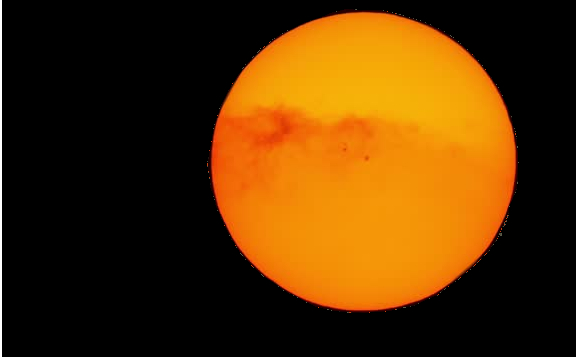
\includegraphics[width=0.4\textwidth]{img/orange.jpg}
		\caption{Наглядное изображение оранжевого круга на черном фоне.}}
\end{figure}

\begin{figure}[ht!]%
    \centering
	\subfloat[A]{{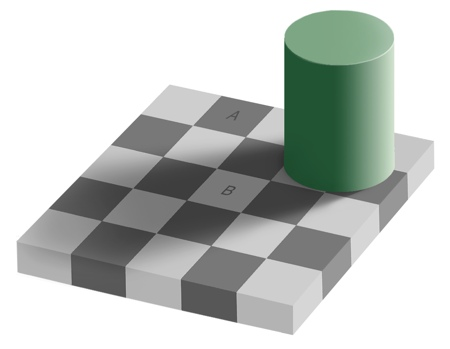
\includegraphics[width=6cm]{img/illusion_1.jpg} }}%
    \qquad
	\subfloat[B]{{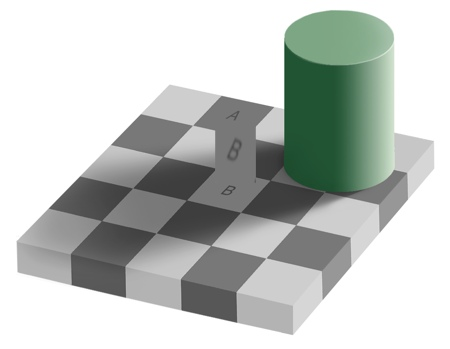
\includegraphics[width=6cm]{img/illusion_2.jpg} }}%
	\caption{Демонстрация психологических факторов человеческого восприятия(рисунок A-квадрат B кажется светлее квадрата A, но на самом деле они одного цвета(рисунок B)).}%
    \label{fig:example}%
\end{figure}

В работе будет рассматриваться первый случай, где не учитываются психологические аспекты человеческого восприятия. Следует выделить четкое понятие доминантного цвета:

\textit{Доминантный(преобладающий) цвет} -- цвет, который представляет группу цветов пикселей, объедененных в единый кластер с помощью квантования. 



\section{ Цвет}
С физической точки зрения цвет представляет собой свет, который, отражаясь от объекта, попадает в глаз человека. Восприятие цвета человеком может зависить от психологического состояния индивида, от местоположения объекта, от строение глаза человека, от окружаещего света и т.д. То есть восприятяие цвета человеком достаточно субъективно. Свет в свою очередь можно описать как волну, длинна которой возбуждает разные рецепторы человеческого глаза. То есть, индивид будет понимать какого цвета объект перед ним в зависимости от того, в какой диапазон попадет длинна волны света, отраженного от этого объекта.

\subsection{ Модели цвета}

Модель цвета -- абстрактная математическая модель представления цветов в виде кортежей чисел.

В какой-то момент необходимо было придумать модель цвета. Описать это явление так, чтобы можно было эффективно и удобно представлять цветовую информацию в цифровом виде. Проблема описания цвета в форме математики была решена еще до появления компьютеров. Одним из первых таких описаний было RGB(Red, green, blue) пространство, идея которого заключалась в представлении всех цветов, различимых человеком, с помощью трех базовых понятий - красного, зеленого и синего. RGB не является одним единственным пространством. Список основных цветовых пространств:
\begin{enumerate}
	\item RGB, sRGB, Adobe RGB
	\item CIEXYZ, CIELAB
	\item CMY(K)
	\item HSL, HSV
\end{enumerate}

$RGB$ -- пространство, строящееся на составление цвета из трех базовых -- красного(Red), синего(Blue) и зеленого(Green). Данную модель часто называют цветовым кубом, потому что каждый базовый параметр цвета, представленного в этой модели, может восприниматься как координата трехмерного пространства.

\begin{figure}[ht!]
	\centering{
		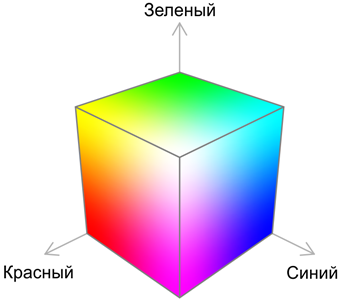
\includegraphics[width=0.4\textwidth]{img/colorCube.png}
		\caption{Представление цветового куба.}}
\end{figure}

Данная модель способна представить 16 777 216(\(2^8 * 2^8 * 2^8\)) цветов.\\

\textit{CIEXYZ(CIE - International Commission on Illumination)} -- модель, которая является экстраполяцией RGB модели. Данная модель охватывает все цвета, видимые человеком. Когда модель RGB расширили до видимых цветов появились отрицательные числа и чтобы избавиться от них были введены мнимые основные цвета X(мнимый красный), Y(мнимый зеленый), Z(мнимый синий).

\textit{CIELAB(L*a*b*)} -- цветовая модель, которая может отображать цвета за пределами, распознаваемыми человеком. Основывается на трех параметрах: L - яркости(Lightness) и двух цветовых каналов a и b. Проблема данного цветового пространства заключается в том, что расстояние между цветами в этой цветовой модели не соответствует цветовому спектру(Например, расстояние от зеленого к зелено-желтому большое в то время как от красного к синиму достаточно маленькое)

\begin{figure}[ht!]
	\centering{
		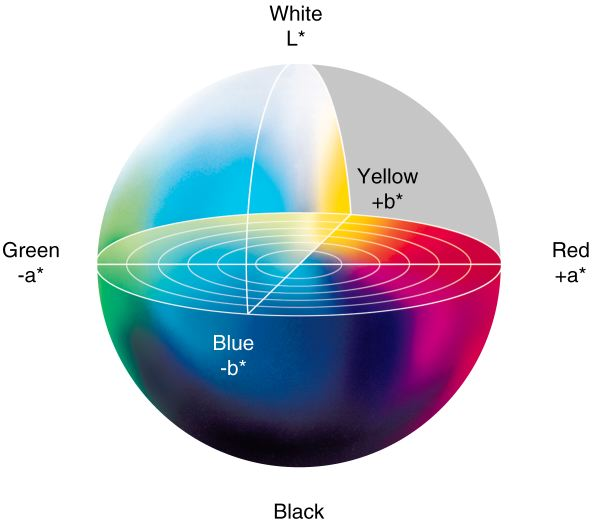
\includegraphics[width=0.4\textwidth]{img/lab.png}
		\caption{Представление цветовой модели CIALAB.}}
\end{figure}

\textit{CMY(K)} -- цветовая модель, аббревиатуру которой можно расшифровать как Cyan(голубой), Magenta(пурпурный), Yellow(желтый), blacK(Key). Данная цветовая модель широко используется в печати документов, изображений. Изначально в данном пространстве исплользовалось только три цвета: cyan, magenta, yellow, с помощью которых можно было получить и черный цвет, смешивая краски. Но это оказалось не эффективно и затратно, поэтому для черного решили ввести отдельный канал, что позволило сэкономить очень много средств.

\begin{figure}[ht!]
	\centering{
		
\includegraphics[width=0.4\textwidth]{img/cmyk.png}
		\caption{Представление цветовой модели CMYK.}}
\end{figure}\\

\textit{YUV, YIQ} -- цветовые модели, где информация о цвете передавалась в виде яркости(Y) и двху цветоразностных сигналов IQ/UV. Благодаря тому, что в Y изображение хранилось в градациях серого, изображение могло подаваться и на старые бесцветные телевизоры.\\

\textit{HSL, HSV} -- цветовые пространства, строящиеся на оттенке(Hue), насещенности(Saturation), яркости(Lightness) или значении(Value).

Яркость(L) и значение(V) -- это разные вещи:\\

\(R, G, B \in [0, 1]\)

\(V = \max{R, G, B}\)

\(L = \frac{1}{2} (\max{R, G, B} + \min{R, G, B})\)\\

Насыщенность у этих моделей тоже разная:\\

S_{HSV} = \frac{\max{R, G, B} - min{R, G, B}}{V}

S_{HSL} = \frac{\max{R, G, B} - min{R, G, B}}{1-|2L-1|}

\begin{figure}[ht!]
	\centering{
		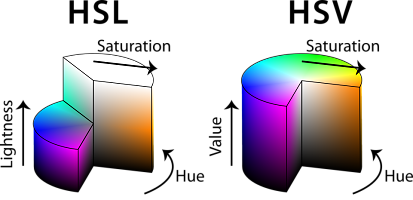
\includegraphics[width=0.4\textwidth]{img/hsl_hsv.png}
		\caption{Представление цветовой модели CIALAB.}}
\end{figure}

\subsection{ Квантование цвета}
Квантование -- разбиение диапазона значений некоторой величины на конечное число уровней и округление этих значений до ближайших к ним уровней.

Квантование цвета в изображении важнейшая задача в поиске преобладающих цветов. Она позваляет уменьшить количество цветов отображаемой картинки. Это активно используется при сжатии, позволяя уменьшить глубину цвета, при добавлении эффектов на изображение. Следующие алгоримы позволяют решить данную задачу:
\begin{enumerate}
	\item Алгоритм равномерного(однородного) квантования.
	\item Алгоритм квантования цветов медианным сечением.
	\item Алгоритмы кластеризации(Например алгоритм k-средних).
\end{enumerate}

\textit{Алгоритм квантования цветов медианным сечением:}

Данный метод заключается в разбиении цветового пространства на параллелепипеды со сторонами, параллельными осям цветового пространства RGB.

Первый шаг заключается в нахождении минимального параллелепипеда, который содержит все цвета, представленые в изображении.

На втором шаге происходит определение самой длинной стороны параллелепипеда и сортировка всех значений вдоль выбранного направления. Далее параллелепипед разделяется по медиане множества значений выбранного направления на две части. Отсюда, получится два параллелепипеда, которые содержат примерно одинаковое количество значений. 

Предыдущая процедура повторяется до тех пор, пока не будет получено N параллелепипедов, где N - количество цветов новой палитры. После этого требуется заполнить палитру цветов, которая будет описывать изображение. Для каждого параллелепипеда нужно рассчитать цвет, который будет представлять его(либо центральная точка параллелепипеда, либо среднее арифметическое значение точек, попавших в него)

На самом изображении остается проанализировать пиксель(найти параллелепипед, в который попадает данная точка) и заменить цвет пикселя на цвет, который представляет весь параллелепипед.

\textit{Алгоритм кластеризации k-средних:}

Метод кластеризации основан на центроидах -- точках, которые представляют собой центр кластера.

Первый шаг алгоритма заключается в инициализации центроидов, количество которых равно N(размер требуемой палитры). Инициализация центроидов очень важный момент, который сильно влияет на работу всего алгоритма. Можно взять случайные центроиды, но это возможно приведет к погрешности.

Далее выделяется два основных шага данного алгоритма: нахождение кластеров, которые определяются путем кратчайшего расстояние от точки до центроида, и рассчитывание центра масс получившихся кластеров, смещение центроидов на полученные центры масс. Эти два шага повторяются до тех пор, пока центроиды не стабилизируются и больше не будут смещаться.

\begin{figure}[ht!]
	\centering{
		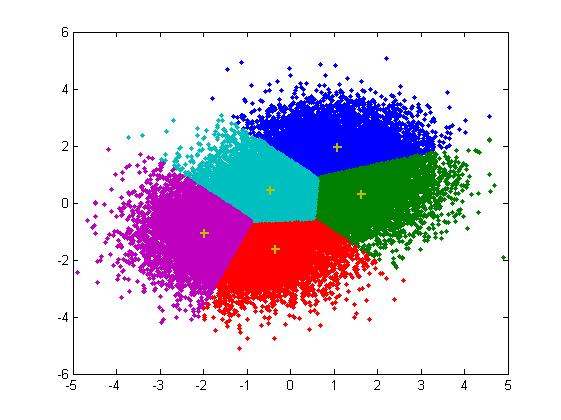
\includegraphics[width=0.4\textwidth]{img/k-means.jpg}
		\caption{Результат работы k-means с представленными центроидами.}}
\end{figure}

\subsection{ Цветовые гистограммы}
Гистограмма -- график статического распределения цифрового изображения с различной яркостью, в котором по горизонтальной оси представлена яркость, а по вертикали -- относительное число пикселей с конкретным значением яркости. С помощью гистограммы определяется насыщенность изображения(либо сумарная, либо разделенная по цветовым каналам).

\begin{figure}[ht!]
	\centering{
		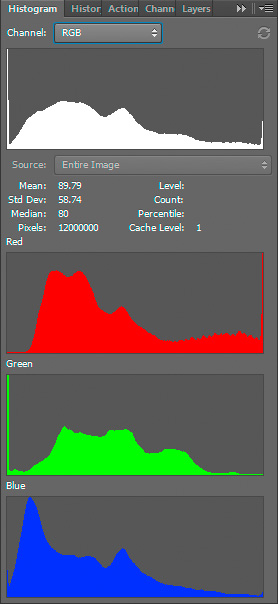
\includegraphics[width=0.4\textwidth]{img/histograms.jpg}
		\caption{Гистограммы, характеризующие изображение в программе Photoshop CS6.}}
\end{figure}

\subsection{ MPEG-7}
MPEG-7 -- стандарт ISO/IEC, разработанный группой MPEG(Moving Picture Experts Group). Аббревиатура расшифровывается как Multimedia Content Description Interface(Мультимедиа-интерфейс для описания содержимого). Имеет цель стандартизировать и описать мультимедийное пространство.

Стандарт состоит из семи частей:
\begin{enumerate}
	\item Системы MPEG-7.
	\item Язык описания определений MPEG-7.
	\item Audio -- дескрипторы и схемы описания аудио материала.
	\item Visual -- дескрипторы и схемы описания визуального материала.
	\item Multimedia Descriptor Schemes -- дескрипторы и схемы описания общих характеристик описания мультимедиа.
	\item Reference Software -- програмные реализации соответствующих частей стандарта.
	\item Conformance -- базовые принципы и процедуры тестирования рабочих характеристик практических реализаций стандарта.
\end{enumerate}

\subsection{ Трехмерное представление цвета}

\section{ Алгоритмы выделения преобладающего цвета}
\subsection{ Histogram algorithms}
\subsection{ GLA(generalized Lloyd Algorithm)}
\subsection{ Clustering algorithms}

\section{ Выбор подходящего алгоритма для решения задачи}

\chapter{ Констукторский раздел}
\label{cha:design}

%\chapter{ Технологический раздел}
\label{cha:design}

%\chapter{Исследовательский раздел}

В данном разделе представлены  результаты сравнения разработанного метода преобразования разработанного метода преобразования LDR видео в HDR с отображением его на LDR мониторе с помощью алгоритмов слияния экспозиций, BMD и BMT, которые являются самыми распространенными среди алгоритмов удаления движущихся объектов с кадров, получением HDR изображения и выравнивании кадров(регистрацией изображений).

Анализ результатов производился на наборе данных, полученных с помощью камеры, способной записывать видео с качеством до 720p 60 кадров в секунду. Технические характеристики устройства, на котором производились вычисления:

\begin{itemize}
    \item процессор Intel Core i7-8550U
    \item оперативная память: 8ГБ
    \item дисковый SSD накопитель, имеющий среднюю скорость считывания - 520 МБ/c, а время доступа 5.78 мс
        \item операционная системя Arch Linux x86\_64 с ядром: 5.0.6-arch1-1-ARCH
\end{itemize}

\section{ Анализ работы построения HDR видео спроектированным методом}

На рисунках \ref{fig:hdr_car_pipeline} и на рисунках \ref{fig:hdr_cafe_pipeline} можно посмотреть результат работы спроектированного метода. Кадры, представленные на рисунках представлены в разрешении 640x480.

\begin{figure}[!tbp]
  \centering
  \begin{subfigure}{.5\textwidth}
    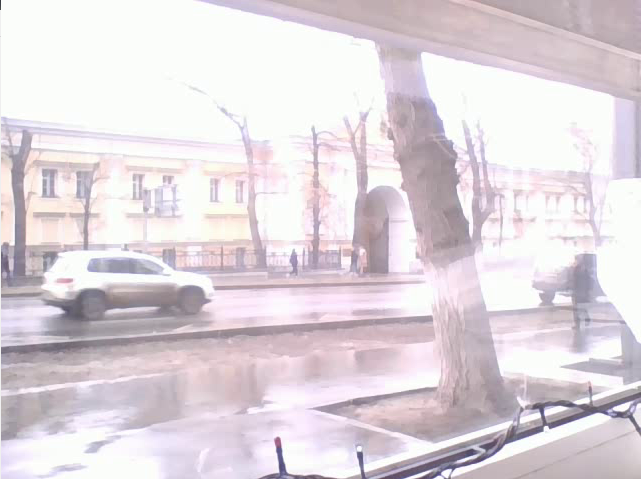
\includegraphics[width=\textwidth]{img/exposure1_car.png}
    \caption{ кадр с завышенной экспозицией}
    \label{fig:exposure1_car}
  \end{subfigure}\hfill
  \begin{subfigure}{.5\textwidth}
    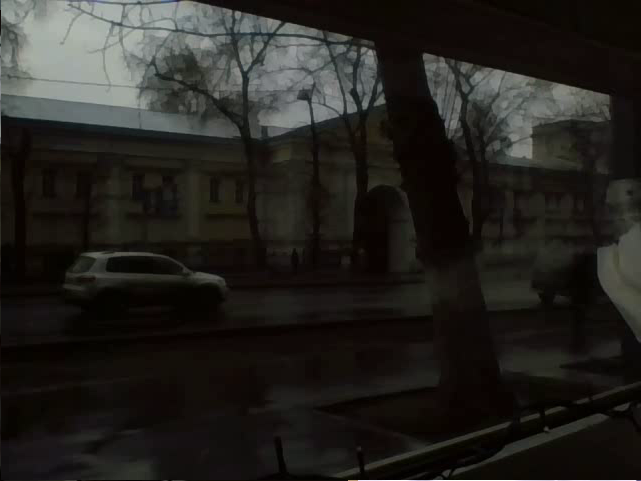
\includegraphics[width=\textwidth]{img/exposure2_car.png}
    \caption{ кадр с заниженной экспозицией}
    \label{fig:exposure2_car}
  \end{subfigure}\hfill
  \begin{subfigure}{1\textwidth}
    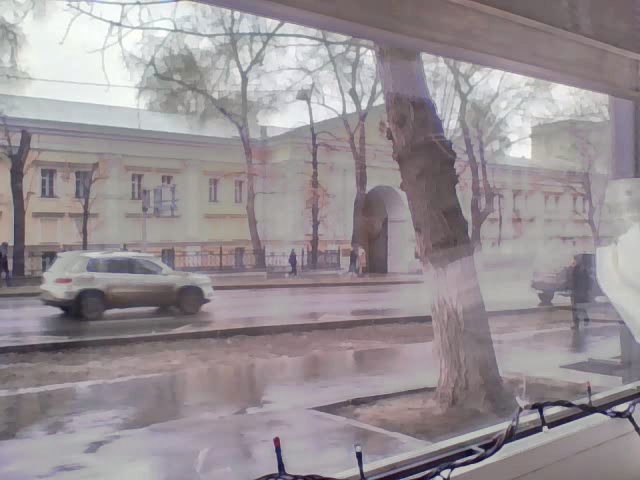
\includegraphics[width=\textwidth]{img/hdr_car_deghost.png}
    \caption{ Полученное HDR изображение}
    \label{fig:hdr_car2}
  \end{subfigure}
  \caption { Результаты обработки двух кадров с разными экспозициями из видео потока(разрешение:640x480).}
  \label{fig:hdr_car_pipeline}
\end{figure}

\begin{figure}[!tbp]
  \centering
  \begin{subfigure}{.5\textwidth}
    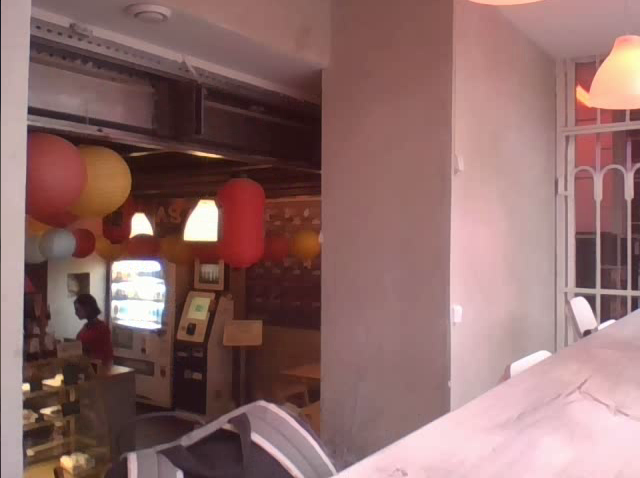
\includegraphics[width=\textwidth]{img/exposure1_cafe.png}
    \caption{ кадр с завышенной экспозицией}
    \label{fig:exposure1_cafe}
  \end{subfigure}\hfill
  \begin{subfigure}{.5\textwidth}
    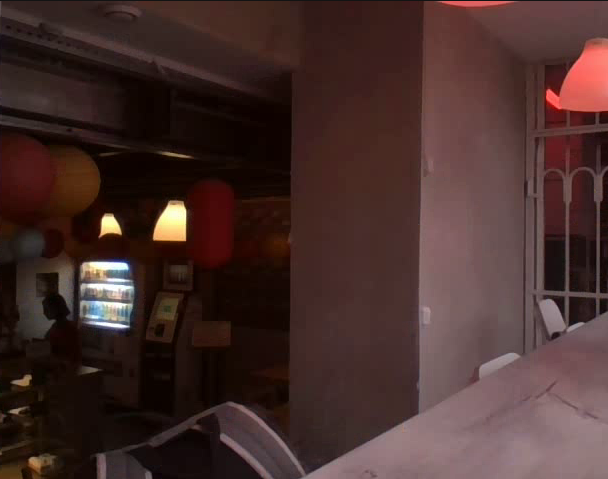
\includegraphics[width=\textwidth]{img/exposure2_cafe.png}
    \caption{ кадр с заниженной экспозицией}
    \label{fig:exposure2_cafe}
  \end{subfigure}\hfill
  \begin{subfigure}{1\textwidth}
    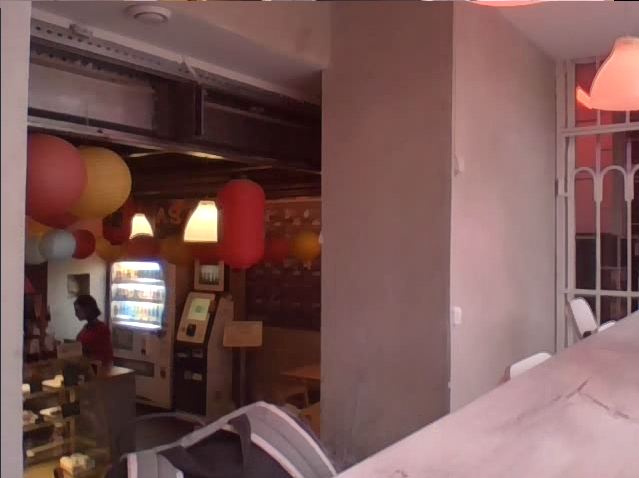
\includegraphics[width=\textwidth]{img/hdr_cafe_deghost.png}
    \caption{ Полученное HDR изображение}
    \label{fig:hdr_cafe_deghost}
  \end{subfigure}
  \caption { Результаты обработки двух кадров с разными экспозициями из видео потока(разрешение:640x480).}
  \label{fig:hdr_cafe_pipeline}
\end{figure}

На рисунках \ref{fig:hdr_street_hd_pipeline} представлены кадры из видео потока и полученное изображение с помощью спроектированного метода в разрешении: 1280x720)

\begin{figure}[!tbp]
  \centering
  \begin{subfigure}{.5\textwidth}
    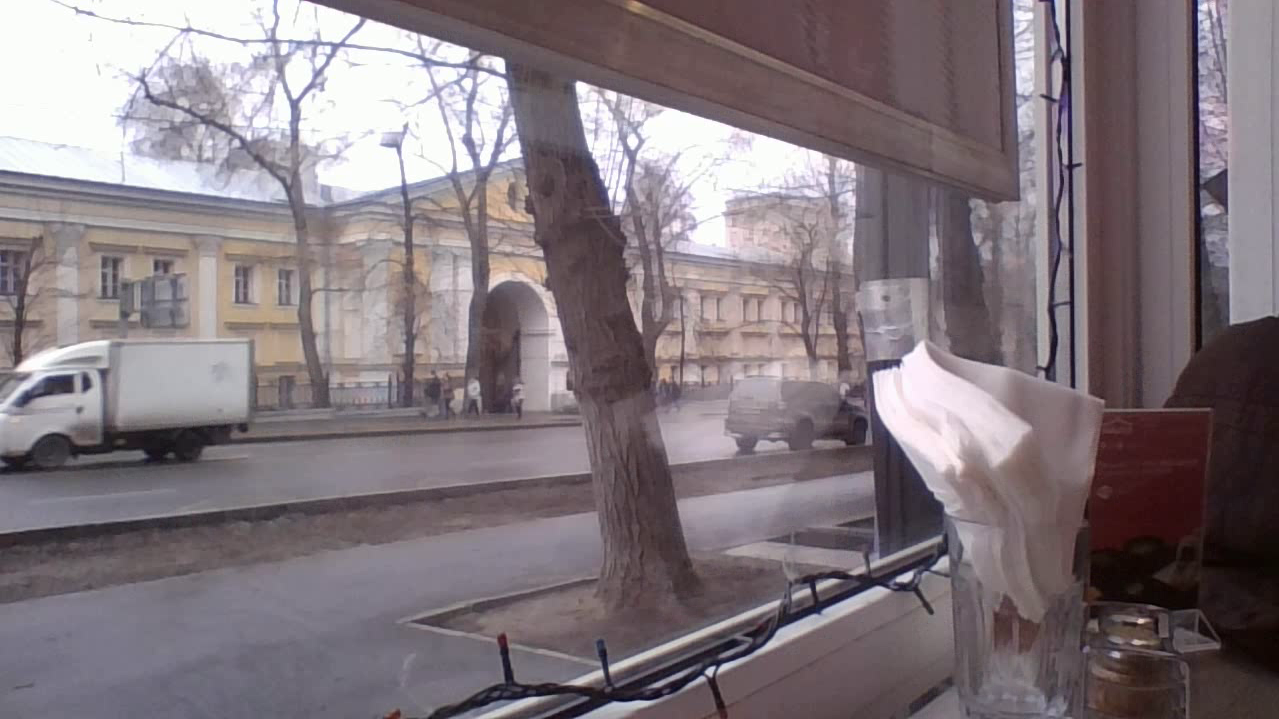
\includegraphics[width=\textwidth]{img/exposure1_street_hd.png}
    \caption{ кадр с завышенной экспозицией}
    \label{fig:exposure1_street_hd}
  \end{subfigure}\hfill
  \begin{subfigure}{.5\textwidth}
    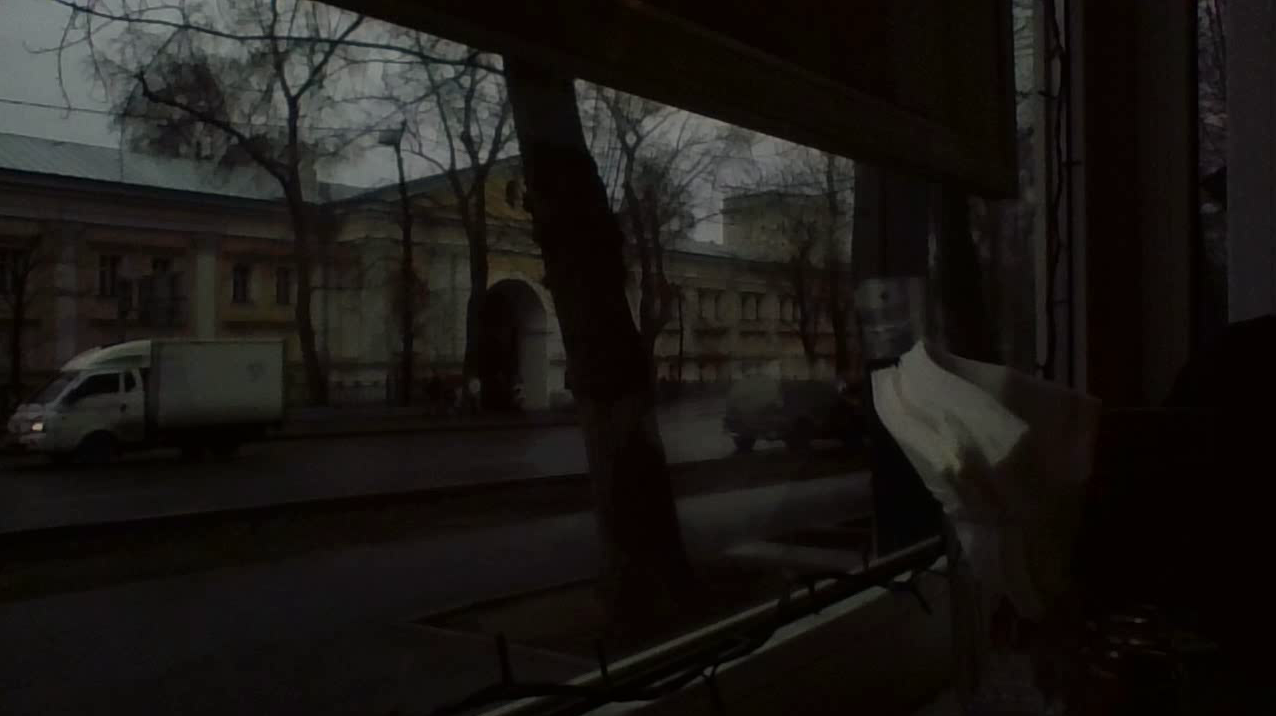
\includegraphics[width=\textwidth]{img/exposure2_street_hd.png}
    \caption{ кадр с заниженной экспозицией}
    \label{fig:exposure2_street_hd}
  \end{subfigure}\hfill
  \begin{subfigure}{1\textwidth}
    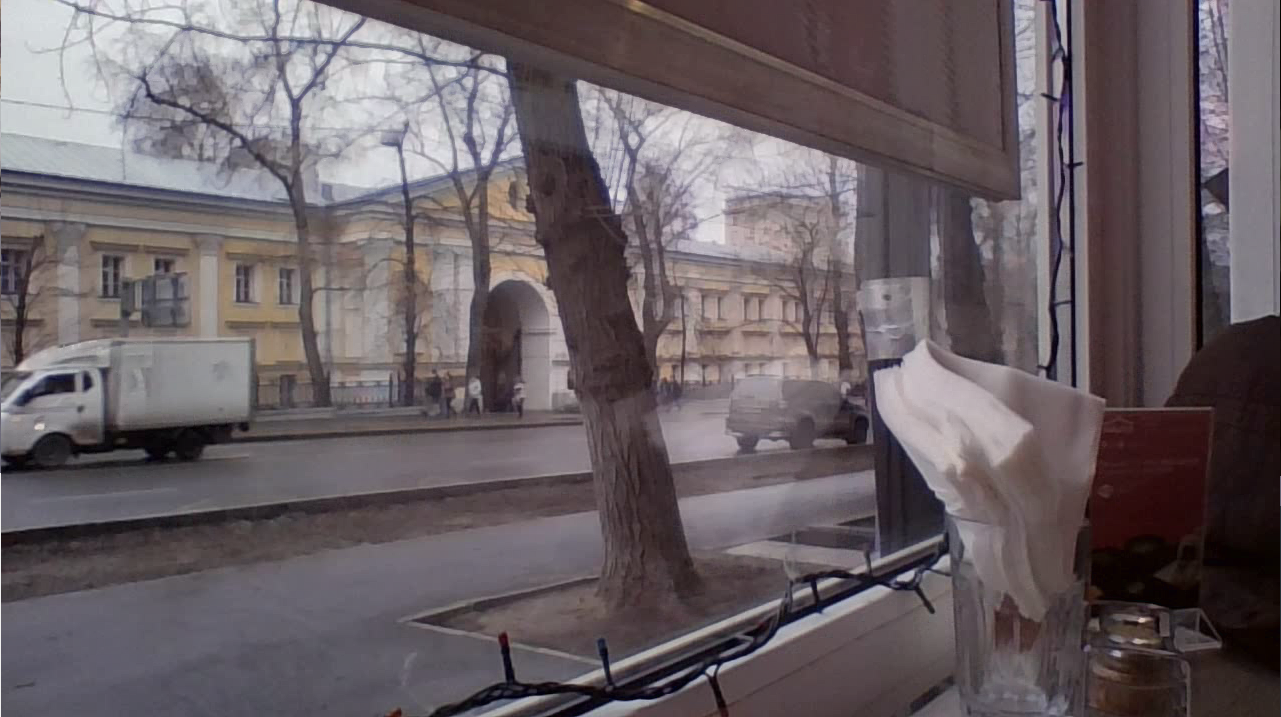
\includegraphics[width=\textwidth]{img/hdr_street_hd.png}
    \caption{ Полученное HDR изображение}
    \label{fig:hdr_street_deghost_hd}
  \end{subfigure}
  \caption { Результаты обработки двух кадров с разными экспозициями из видео потока(разрешение:1280x720).}
  \label{fig:hdr_street_hd_pipeline}
\end{figure}


\section{ Анализ работы определения зон движения и их удаления}



\backmatter %% Здесь заканчивается нумерованная часть документа и начинаются ссылки и
            %% заключение

%\Conclusion % заключение к отчёту

В результате выполнения крусового проекта были получены следующие основные результаты:


% % Список литературы при помощи BibTeX
% Юзать так:
%
% pdflatex rpz
% bibtex rpz
% pdflatex rpz

\bibliographystyle{gost780u}
\bibliography{rpz}


%%% Local Variables: 
%%% mode: latex
%%% TeX-master: "rpz"
%%% End: 


%\appendix   % Тут идут приложения

%%\chapter{Картинки}
%\label{cha:appendix1}

%\begin{figure}
%\centering
%\caption{Картинка в приложении. Страшная и ужасная.}
%\end{figure}

%%% Local Variables: 
%%% mode: latex
%%% TeX-master: "rpz"
%%% End: 

%%\chapter{Еще картинки}
%\label{cha:appendix2}

%\begin{figure}
%\centering
%\caption{Еще одна картинка, ничем не лучше предыдущей. Но %надо же как-то заполнить место.}
%\end{figure}

%%% Local Variables: 
%%% mode: latex
%%% TeX-master: "rpz"
%%% End: 


\end{document}

%%% Local Variables:
%%% mode: latex
%%% TeX-master: t
%%% End:
